\documentclass[a4paper, 12pt]{article}

\usepackage[utf8]{inputenc}
\usepackage{latexsym,amsfonts,amssymb,amsthm,amsmath}
\usepackage{setspace}
\usepackage{physics}
\usepackage{graphicx}
\usepackage{newtxtext}
\usepackage{extsizes}
\setlength{\parindent}{0in}
\setlength{\oddsidemargin}{0in}
\setlength{\textwidth}{6.5in}
\setlength{\textheight}{8.8in}
\setlength{\topmargin}{0in}
\setlength{\headheight}{8pt}

\onehalfspacing


\title{
  \vspace{-1.5cm}
  \textbf{Nonparametric tests\\(Pearson's Chi-square test)}
  \vspace{-1.5cm}
}
\date{}

\begin{document}

\maketitle

\section{Tests of goodness of fit}

In the first part of this lecture, we will consider tests that check whether
given data are in accordance with a certain assumption about the population
feature distribution.

Consider the case of testing a simple null versus a complex alternative
hypothesis:
\[
H_0 (F = F_0) \quad \text{vs.} \quad H_a (F \neq F_0)
\]

The real line $\mathbb{R}$ is split into $r$ classes $S_1, \dots, S_r$, i.e., into $r$ pairwise disjoint sets, such that the probabilities are all positive.\

Then, if $n$ observations are made and if the null hypothesis is true, the expected frequency $E_k$ of the observations from the sample that are in the class $S_k$ is equal to $np_k$, for $k = 1, \dots, r$.

Let $(X_1, \dots, X_n)$ be a random sample for $X$ and let $N_1, \dots, N_r$ be the observed sample frequencies for the classes $S_1, \dots, S_r$ (frequencies of the sample data in each of the classes).

\section{Pearson $\mathcal{X}^2-$tests}

As a measure of the differences between the observed sample frequencies $N_1, \dots, N_r$ and the assumed (expected) frequencies $np_1, \dots, np_r$, when the null hypothesis is true, the following statistic, known as Pearson's $\chi^2$, is used:

\[
\mathcal{X}^2 = \sum_{k=1}^{r} \frac{(N_k - np_k)^2}{np_k}
\]

\begin{itemize}
    \item It is shown that, when the null hypothesis is true, this statistic has an approximate $\chi^2$ distribution with $r - p - 1$ degrees of freedom, where $p$ is the number of unknown parameters in the hypothesized distribution that will be estimated from the sample. Thus, we need $r > p + 1$.
    \item For example, if the distribution in the null hypothesis is $N(\mu, \sigma^2)$ and both parameters are unknown, the statistic $\chi^2$ will have an approximately $\chi^2$ distribution with $r - 2 - 1$ degrees of freedom.
    \item The unknown parameters are estimated by estimators obtained with the methods we studied.
\end{itemize}


These estimators for the unknown parameters are obtained by both methods (both the method of moments and the method of maximum likelihood), except for the estimator for the unknown parameter $m$ for the binomial distribution which is obtained by the method of moments.

\begin{figure}[h!]
  \centering
  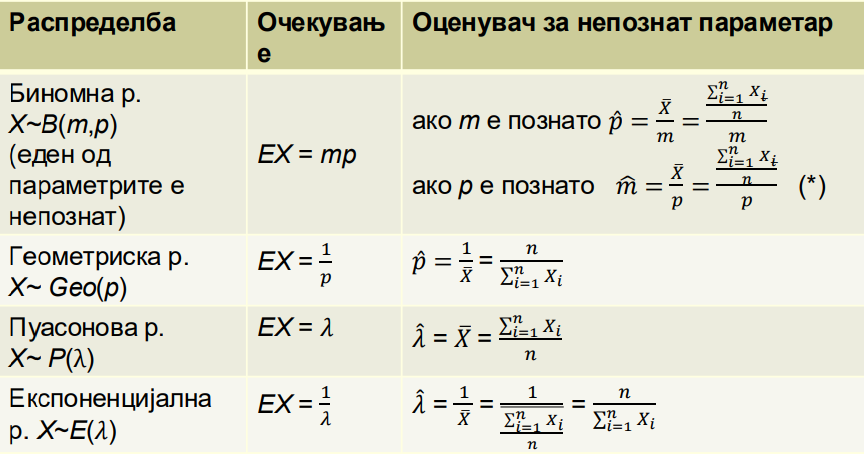
\includegraphics[width=0.8\textwidth]{image_2.png}
  \caption{}
  \label{fig:example_image}
\end{figure}

Note(*). Pay attention to examples in which the binomial distribution is denoted by $B(n,p)$. Here $n$ should not be confused with the sample size, for which in such a case it is desirable to use a different notation.

\begin{figure}[h!]
  \centering
  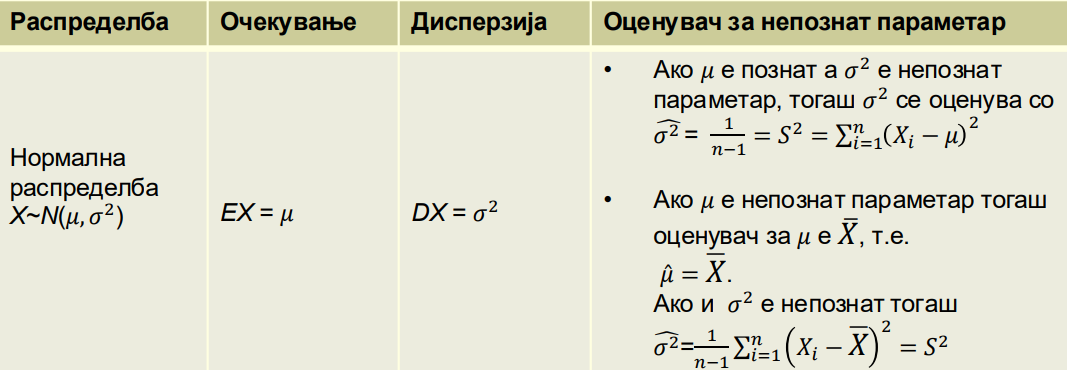
\includegraphics[width=0.8\textwidth]{image.png}
  \caption{}
  \label{fig:example_image}
\end{figure}

As an estimator for $\sigma^2$ we use the variance of the sample.

\section{Pearson $\chi^2$-test}  

When applying this test, we should pay attention to the size of the expected frequencies.  
If the expected frequencies are too small, the test statistic will not reflect the difference of the observed from the expected frequencies, but only the small value of the expected frequencies.  \\

Therefore, for each of the classes, the expected frequency should be at least 5.  
Since the size of the classes need not be equal, if the expected frequency for any of the classes is less than 5, then that class is merged with a neighbouring class.  \\

Thereby, the expected (observed) frequency of the newly formed class is obtained by summing the expected (observed) frequencies of the merged classes.  
With this, the number of classes $r$ will decrease by 1.\\


If the hypothesis $H_0$ is correct, we expect the differences between the sample frequencies and the predicted frequencies to be small.  \\

Therefore, for large values of the statistic we will reject the null hypothesis as false.  \\

Therefore, the critical domain of the test is given by
\[
C = \left(X_{\alpha, r-p-1}, +\infty \right).
\]

\begin{figure}[h]
  \centering
  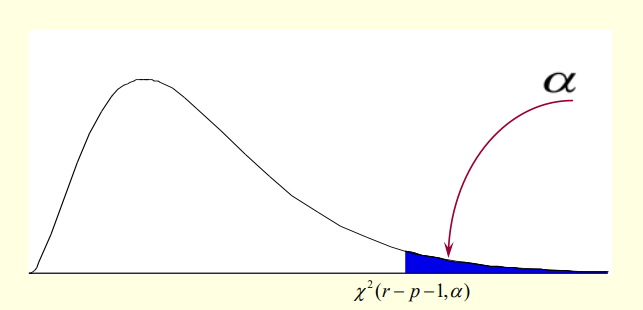
\includegraphics[width=0.8\textwidth]{image_3.png}
  \caption{}
  \label{fig:example_image}
\end{figure}

\textbf{Example 1: } Four coins are tossed 160 times. The following frequencies of appearances on the tails were observed:


\begin{table}[h!]
\centering
\begin{tabular}{lllllll}
\textbf{k}     & \textbf{0} & \textbf{1} & \textbf{2} & \textbf{3} & \textbf{4} & \textbf{Total} \\
\textbf{$N_k$} & 6          & 34         & 67         & 41         & 12         & 160           
\end{tabular}
\end{table}

Check with 5\% significance level if these are fair coins!
If the coins are fair and $X$ is the number of appearances of tails, we expect a binomial distribution, i.e., $X \sim B(4,1/2)$.


\textbf{Example 2: Binomial distribution, unknown $p$}
Random samples of 20 pieces are taken from a large number of
products. The experiment is repeated 100 times. We want to
estimate the probability of defective product appearance and
whether the number of defective products has a binomial
distribution. The observed frequencies of defective products in
each of the selected samples of 20 products are:

\begin{table}[h!]
\centering
\begin{tabular}{|l|l|l|l|l|l|l|l|l|}
\hline
\textbf{k}     & \textbf{0} & \textbf{1} & \textbf{2} & \textbf{3} & \textbf{4} & \textbf{5} & \textbf{6} & \textbf{Total} \\ \hline
\textbf{$N_k$} & 14         & 25         & 27         & 23         & 7          & 3          & 1          & 100            \\ \hline
\end{tabular}
\end{table}

With a significance level of 5\% check whether the number of
defective products has a binomial distribution.


\textbf{Example 3: Poisson distribution}

The following table shows observed frequencies of the number
of machine breakdowns in an industrial plant.

\begin{table}[h!]
\centering
\begin{tabular}{|l|l|l|l|l|l|l|l|l|l|l|l|l|}
\hline
\textbf{Daily breakdowns: k} & \textbf{$\leq$5} & \textbf{6} & \textbf{7} & \textbf{8} & \textbf{9} & \textbf{10} & \textbf{11} & \textbf{12} & \textbf{13} & \textbf{14} & \textbf{15} & \textbf{$\geq$16} \\ \hline
\textbf{Freq: $N_k$}         & 11               & 13         & 20         & 18         & 27         & 34          & 28          & 12          & 13          & 10          & 7           & 7                 \\ \hline
\end{tabular}
\end{table}

The hypothesis that the distribution of the number of
breakdowns during the day is Poisson distribution or $H_0$ ($X\sim P(\lambda)$).


\textbf{Example 4: Normal distribution}


Long-term statistics show that the height of students at a
university has a normal distribution with mean $\mu = 173 cm$ and
standard deviation $\sigma = 7 cm$. A random sample of 100 was taken
from one generation of students. The obtained measurements are
distributed in classes as in the table:

\begin{table}[h!]
\centering
\begin{tabular}{|l|l|l|l|l|l|l|l|}
\hline
\textbf{$S_k$} & {[}152, 160) & {[}160, 166) & {[}166, 172) & {[}172, 178) & {[}178, 184) & {[}184, 190) & \textbf{Total} \\ \hline
\textbf{$N_k$} & 5            & 17           & 38           & 25           & 9            & 6            & 100            \\ \hline
\end{tabular}
\end{table}

At a 5\% level of significance, check whether the distribution is
normal with mean $\mu = 173 cm$ and standard deviation $\sigma = 7 cm$.


\section{Testing the independence of two categorical
features}

Pearson's Chi-square test is also used in the analysis of relationships between categorical features.\\

Often, $n$ elements of a sample can be classified according to two different criteria. We may then be interested in whether the two classification methods are independent. For example, we might take the population of engineering graduates, and determine whether the starting salary is independent of academic discipline. \\ 

So, the same individuals (elements) are assigned two qualitative characteristics, $X$ and $Y$. Let the categories of $X$ be $A_1, A_2, \dots, A_r$, and the categories of $Y$ be $B_1, B_2, \dots, B_k$. We want to test the hypothesis:  
\[
H_0: \text{The features } X \text{ and } Y \text{ are independent}
\]  
\[
H_a: \text{The features } X \text{ and } Y \text{ are not independent}
\]

\subsection{Contingency tables}

If the size of the sample (observed individuals) is $n$, a table is formed with $r$ rows corresponding to the categories of $X$ and $k$ columns corresponding to the categories of $Y$. In each $(i,j)$ field of the table, the observed frequency $n_{ij}$ is recorded for the category $A_i$ of $X$ and category $B_j$ of $Y$, i.e., the number of individuals (elements) belonging to the category $A_i$ of $X$ and the category $B_j$ of $Y$.\\

These tables are called contingency tables.

\begin{figure}[h!]
  \centering
  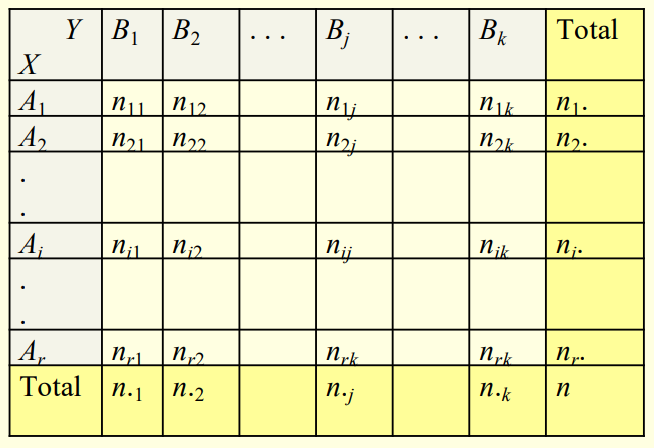
\includegraphics[width=0.5\textwidth]{image_4.png}
  \caption{}
  \label{fig:example_image}
\end{figure}

\[n_{i.} = \sum_{s=1}^{k}n_{is}\]
\[n_{.j} = \sum_{t=1}^{r}n_{ij}\]
\[n =  \sum_{i=1}^{r}\sum_{j=1}^{k}n_{ij}\]

\subsection{Chi-square test for independence}

Let $p_{ij}$ be the probability a random chosen element to be in category $A_i$ of $X$ and category $B_j$ of $Y$ i.e. $p_{ij}=P(A_i\cap B_j)$\\


If $H_0$ is correct then $p_{ij} = P(A_i \cap B_j)=p_{i.}p_{.j}$, where $p_{i.}=P(A_i)$ and $p_{.j}=P(B_j)$\\

The estimators for $p_{i.}$ and $p_{.j}$ are

\[ \hat{p_{i.}} = \frac{n_{i.}}{n} \quad \text{and} \quad \hat{p_{.j}} = \frac{n_{.j}}{n} \]

Therefor if $H_0$ is correct the expected frequency in the fied $(i,j)$ is:

\[ E_{ij} = np_{ij} = \frac{n_{i.} \cdot n_{.j}}{n} \]

For large values of n, when $H_0$ is correct statistic

\[ \mathcal{X}^2 = \sum_{i=1}^{r}\sum_{j=1}^{k} \frac{n_{ij}-E_{ij}}{E_{ij}} 
= \sum_{i=1}^{r}\sum_{j=1}^{k} \frac{n_{ij}-\frac{n_{i.} \cdot n_{.j}}{n}}{\frac{n_{i.} \cdot n_{.j}}{n}} \]

has $\mathcal{X}^2$ distribution with $(r-1)(k-1)$ degrees of freedom.\\

And here the null hypothesis is rejected if the calculated statitstic value is greater than the critical value $\mathcal{X}^2_{\alpha, (r-1)(k-1)}$ which is read from the table.\\

\textbf{Note}: The pearson test is used when the expected frequencies in each cell of the contingency table is at least 5. If this is not met, other tests are recommended.

\newpage

\textbf{Example} With a significance level of $\alpha = 0.05$, test the hypothesis that the car
model of the Peugeot brand does not depend on the gender of the
owner. The results obtained by examining 350 randomly selected car
owners are given in the following contingency table:

\begin{table}[h!]
\centering
\begin{tabular}{|l|l|l|l|}
\hline
\textbf{X\textbackslash{}Y} & \textbf{Peugeot 106} & \textbf{Peugeot 206} & \textbf{Peugeot 306} \\ \hline
\textbf{male}               & 40                   & 80                   & 30                   \\ \hline
\textbf{female}             & 30                   & 120                  & 50                   \\ \hline
\end{tabular}
\end{table}

\subsubsection{Simplifying the Chi-Squared statistic}

With simple algebraic transformations, the formula for the Chi-Squared
statistic can be brought to a form that is more convenient for
calculation. Namely,

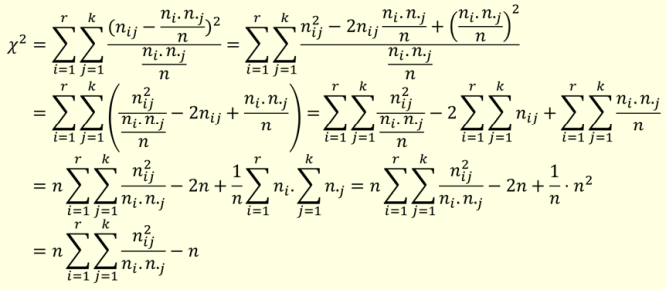
\includegraphics[width=0.9\textwidth]{image_6.png}

\subsection{Contingency factor (coefficient)}

An important measure of the degree of association or
dependence of features in a contingency table is given by the
so-called contingency coefficient, which is calculated as
follows.


\[ C = \sqrt{\frac{\mathcal{X}^2}{\mathcal{X}^2+n}} \]

The higher the values of $C$, the higher the degree of
association. Thus, the value of $C$ never exceeds 1.

\tableofcontents
\end{document}